\documentclass[1p]{elsarticle_modified}
%\bibliographystyle{elsarticle-num}

%\usepackage[colorlinks]{hyperref}
%\usepackage{abbrmath_seonhwa} %\Abb, \Ascr, \Acal ,\Abf, \Afrak
\usepackage{amsfonts}
\usepackage{amssymb}
\usepackage{amsmath}
\usepackage{amsthm}
\usepackage{scalefnt}
\usepackage{amsbsy}
\usepackage{kotex}
\usepackage{caption}
\usepackage{subfig}
\usepackage{color}
\usepackage{graphicx}
\usepackage{xcolor} %% white, black, red, green, blue, cyan, magenta, yellow
\usepackage{float}
\usepackage{setspace}
\usepackage{hyperref}

\usepackage{tikz}
\usetikzlibrary{arrows}

\usepackage{multirow}
\usepackage{array} % fixed length table
\usepackage{hhline}

%%%%%%%%%%%%%%%%%%%%%
\makeatletter
\renewcommand*\env@matrix[1][\arraystretch]{%
	\edef\arraystretch{#1}%
	\hskip -\arraycolsep
	\let\@ifnextchar\new@ifnextchar
	\array{*\c@MaxMatrixCols c}}
\makeatother %https://tex.stackexchange.com/questions/14071/how-can-i-increase-the-line-spacing-in-a-matrix
%%%%%%%%%%%%%%%

\usepackage[normalem]{ulem}

\newcommand{\msout}[1]{\ifmmode\text{\sout{\ensuremath{#1}}}\else\sout{#1}\fi}
%SOURCE: \msout is \stkout macro in https://tex.stackexchange.com/questions/20609/strikeout-in-math-mode

\newcommand{\cancel}[1]{
	\ifmmode
	{\color{red}\msout{#1}}
	\else
	{\color{red}\sout{#1}}
	\fi
}

\newcommand{\add}[1]{
	{\color{blue}\uwave{#1}}
}

\newcommand{\replace}[2]{
	\ifmmode
	{\color{red}\msout{#1}}{\color{blue}\uwave{#2}}
	\else
	{\color{red}\sout{#1}}{\color{blue}\uwave{#2}}
	\fi
}

\newcommand{\Sol}{\mathcal{S}} %segment
\newcommand{\D}{D} %diagram
\newcommand{\A}{\mathcal{A}} %arc


%%%%%%%%%%%%%%%%%%%%%%%%%%%%%5 test

\def\sl{\operatorname{\textup{SL}}(2,\Cbb)}
\def\psl{\operatorname{\textup{PSL}}(2,\Cbb)}
\def\quan{\mkern 1mu \triangleright \mkern 1mu}

\theoremstyle{definition}
\newtheorem{thm}{Theorem}[section]
\newtheorem{prop}[thm]{Proposition}
\newtheorem{lem}[thm]{Lemma}
\newtheorem{ques}[thm]{Question}
\newtheorem{cor}[thm]{Corollary}
\newtheorem{defn}[thm]{Definition}
\newtheorem{exam}[thm]{Example}
\newtheorem{rmk}[thm]{Remark}
\newtheorem{alg}[thm]{Algorithm}

\newcommand{\I}{\sqrt{-1}}
\begin{document}

%\begin{frontmatter}
%
%\title{Boundary parabolic representations of knots up to 8 crossings}
%
%%% Group authors per affiliation:
%\author{Yunhi Cho} 
%\address{Department of Mathematics, University of Seoul, Seoul, Korea}
%\ead{yhcho@uos.ac.kr}
%
%
%\author{Seonhwa Kim} %\fnref{s_kim}}
%\address{Center for Geometry and Physics, Institute for Basic Science, Pohang, 37673, Korea}
%\ead{ryeona17@ibs.re.kr}
%
%\author{Hyuk Kim}
%\address{Department of Mathematical Sciences, Seoul National University, Seoul 08826, Korea}
%\ead{hyukkim@snu.ac.kr}
%
%\author{Seokbeom Yoon}
%\address{Department of Mathematical Sciences, Seoul National University, Seoul, 08826,  Korea}
%\ead{sbyoon15@snu.ac.kr}
%
%\begin{abstract}
%We find all boundary parabolic representation of knots up to 8 crossings.
%
%\end{abstract}
%\begin{keyword}
%    \MSC[2010] 57M25 
%\end{keyword}
%
%\end{frontmatter}

%\linenumbers
%\tableofcontents
%
\newcommand\colored[1]{\textcolor{white}{\rule[-0.35ex]{0.8em}{1.4ex}}\kern-0.8em\color{red} #1}%
%\newcommand\colored[1]{\textcolor{white}{ #1}\kern-2.17ex	\textcolor{white}{ #1}\kern-1.81ex	\textcolor{white}{ #1}\kern-2.15ex\color{red}#1	}

{\Large $\underline{11n_{87}~(K11n_{87})}$}

\setlength{\tabcolsep}{10pt}
\renewcommand{\arraystretch}{1.6}
\vspace{1cm}\begin{tabular}{m{100pt}>{\centering\arraybackslash}m{274pt}}
\multirow{5}{120pt}{
	\centering
	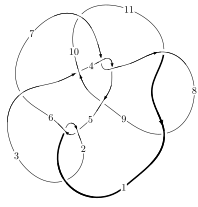
\includegraphics[width=112pt]{../../../GIT/diagram.site/Diagrams/png/703_11n_87.png}\\
\ \ \ A knot diagram\footnotemark}&
\allowdisplaybreaks
\textbf{Linearized knot diagam} \\
\cline{2-2}
 &
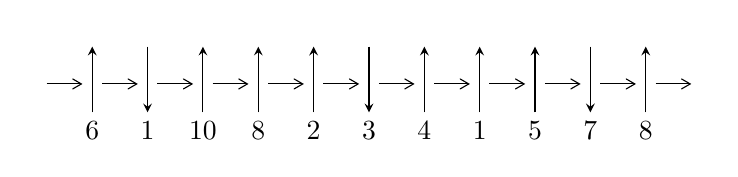
\begin{tikzpicture}[x=20pt, y=17pt]
	% nodes
	\node (C0) at (0, 0) {};
	\node (C1) at (1, 0) {};
	\node (C1U) at (1, +1) {};
	\node (C1D) at (1, -1) {6};

	\node (C2) at (2, 0) {};
	\node (C2U) at (2, +1) {};
	\node (C2D) at (2, -1) {1};

	\node (C3) at (3, 0) {};
	\node (C3U) at (3, +1) {};
	\node (C3D) at (3, -1) {10};

	\node (C4) at (4, 0) {};
	\node (C4U) at (4, +1) {};
	\node (C4D) at (4, -1) {8};

	\node (C5) at (5, 0) {};
	\node (C5U) at (5, +1) {};
	\node (C5D) at (5, -1) {2};

	\node (C6) at (6, 0) {};
	\node (C6U) at (6, +1) {};
	\node (C6D) at (6, -1) {3};

	\node (C7) at (7, 0) {};
	\node (C7U) at (7, +1) {};
	\node (C7D) at (7, -1) {4};

	\node (C8) at (8, 0) {};
	\node (C8U) at (8, +1) {};
	\node (C8D) at (8, -1) {1};

	\node (C9) at (9, 0) {};
	\node (C9U) at (9, +1) {};
	\node (C9D) at (9, -1) {5};

	\node (C10) at (10, 0) {};
	\node (C10U) at (10, +1) {};
	\node (C10D) at (10, -1) {7};

	\node (C11) at (11, 0) {};
	\node (C11U) at (11, +1) {};
	\node (C11D) at (11, -1) {8};
	\node (C12) at (12, 0) {};

	% arrows
	\draw[->,>={angle 60}]
	(C0) edge (C1) (C1) edge (C2) (C2) edge (C3) (C3) edge (C4) (C4) edge (C5) (C5) edge (C6) (C6) edge (C7) (C7) edge (C8) (C8) edge (C9) (C9) edge (C10) (C10) edge (C11) (C11) edge (C12) ;	\draw[->,>=stealth]
	(C1D) edge (C1U) (C2U) edge (C2D) (C3D) edge (C3U) (C4D) edge (C4U) (C5D) edge (C5U) (C6U) edge (C6D) (C7D) edge (C7U) (C8D) edge (C8U) (C9D) edge (C9U) (C10U) edge (C10D) (C11D) edge (C11U) ;
	\end{tikzpicture} \\
\hhline{~~} \\& 
\textbf{Solving Sequence} \\ \cline{2-2} 
 &
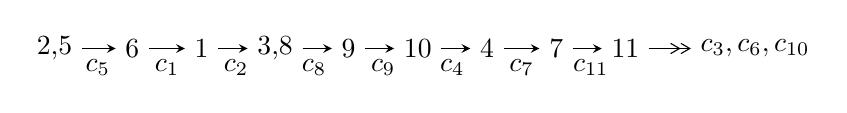
\begin{tikzpicture}[x=25pt, y=7pt]
	% node
	\node (A0) at (-1/8, 0) {2,5};
	\node (A1) at (1, 0) {6};
	\node (A2) at (2, 0) {1};
	\node (A3) at (49/16, 0) {3,8};
	\node (A4) at (33/8, 0) {9};
	\node (A5) at (41/8, 0) {10};
	\node (A6) at (49/8, 0) {4};
	\node (A7) at (57/8, 0) {7};
	\node (A8) at (65/8, 0) {11};
	\node (C1) at (1/2, -1) {$c_{5}$};
	\node (C2) at (3/2, -1) {$c_{1}$};
	\node (C3) at (5/2, -1) {$c_{2}$};
	\node (C4) at (29/8, -1) {$c_{8}$};
	\node (C5) at (37/8, -1) {$c_{9}$};
	\node (C6) at (45/8, -1) {$c_{4}$};
	\node (C7) at (53/8, -1) {$c_{7}$};
	\node (C8) at (61/8, -1) {$c_{11}$};
	\node (A9) at (10, 0) {$c_{3},c_{6},c_{10}$};

	% edge
	\draw[->,>=stealth]	
	(A0) edge (A1) (A1) edge (A2) (A2) edge (A3) (A3) edge (A4) (A4) edge (A5) (A5) edge (A6) (A6) edge (A7) (A7) edge (A8) ;
	\draw[->>,>={angle 60}]	
	(A8) edge (A9);
\end{tikzpicture} \\ 

\end{tabular} \\

\footnotetext{
The image of knot diagram is generated by the software ``\textbf{Draw programme}" developed by Andrew Bartholomew(\url{http://www.layer8.co.uk/maths/draw/index.htm\#Running-draw}), where we modified some parts for our purpose(\url{https://github.com/CATsTAILs/LinksPainter}).
}\phantom \\ \newline 
\centering \textbf{Ideals for irreducible components\footnotemark of $X_{\text{par}}$} 
 
\begin{align*}
I^u_{1}&=\langle 
u^{13}- u^{12}+4 u^{11}-3 u^{10}+7 u^9-6 u^8+7 u^7-7 u^6+4 u^5-5 u^4+2 u^3-2 u^2+b+2 u-1,\\
\phantom{I^u_{1}}&\phantom{= \langle  }- u^{15}+3 u^{14}+\cdots+2 a-4 u,\;u^{16}-3 u^{15}+\cdots-6 u+2\rangle \\
I^u_{2}&=\langle 
- u^6 a- u^5 a-3 u^4 a+u^5-2 u^3 a+u^4-3 u^2 a+3 u^3-2 a u+2 u^2+b- a+3 u+2,\\
\phantom{I^u_{2}}&\phantom{= \langle  }-2 u^7 a+2 u^7-4 u^5 a+2 u^6+5 u^5-3 u^3 a+3 u^4-2 u^2 a+4 u^3+a^2+2 a u+3 u^2-2 a-2 u,\\
\phantom{I^u_{2}}&\phantom{= \langle  }u^8+u^7+3 u^6+2 u^5+3 u^4+2 u^3-1\rangle \\
I^u_{3}&=\langle 
b-1,\;u^3-2 u^2+2 a-2,\;u^4+2 u^2+2\rangle \\
\\
I^v_{1}&=\langle 
a,\;b+1,\;v+1\rangle \\
\end{align*}
\raggedright * 4 irreducible components of $\dim_{\mathbb{C}}=0$, with total 37 representations.\\
\footnotetext{All coefficients of polynomials are rational numbers. But the coefficients are sometimes approximated in decimal forms when there is not enough margin.}
\newpage
\renewcommand{\arraystretch}{1}
\centering \section*{I. $I^u_{1}= \langle u^{13}- u^{12}+\cdots+b-1,\;- u^{15}+3 u^{14}+\cdots+2 a-4 u,\;u^{16}-3 u^{15}+\cdots-6 u+2 \rangle$}
\flushleft \textbf{(i) Arc colorings}\\
\begin{tabular}{m{7pt} m{180pt} m{7pt} m{180pt} }
\flushright $a_{2}=$&$\begin{pmatrix}0\\u\end{pmatrix}$ \\
\flushright $a_{5}=$&$\begin{pmatrix}1\\0\end{pmatrix}$ \\
\flushright $a_{6}=$&$\begin{pmatrix}1\\- u^2\end{pmatrix}$ \\
\flushright $a_{1}=$&$\begin{pmatrix}- u\\u^3+u\end{pmatrix}$ \\
\flushright $a_{3}=$&$\begin{pmatrix}- u^3\\u^5+u^3+u\end{pmatrix}$ \\
\flushright $a_{8}=$&$\begin{pmatrix}\frac{1}{2} u^{15}-\frac{3}{2} u^{14}+\cdots-3 u^2+2 u\\- u^{13}+u^{12}+\cdots-2 u+1\end{pmatrix}$ \\
\flushright $a_{9}=$&$\begin{pmatrix}-\frac{1}{2} u^{15}+\frac{3}{2} u^{14}+\cdots-3 u+2\\u^{13}- u^{12}+\cdots+u-1\end{pmatrix}$ \\
\flushright $a_{10}=$&$\begin{pmatrix}-\frac{1}{2} u^{15}+\frac{3}{2} u^{14}+\cdots-2 u+1\\u^{13}- u^{12}+\cdots+u-1\end{pmatrix}$ \\
\flushright $a_{4}=$&$\begin{pmatrix}-\frac{1}{2} u^{15}+\frac{3}{2} u^{14}+\cdots-2 u+1\\- u^{15}+2 u^{14}+\cdots-2 u+1\end{pmatrix}$ \\
\flushright $a_{7}=$&$\begin{pmatrix}- u^6- u^4+1\\u^8+2 u^6+2 u^4\end{pmatrix}$ \\
\flushright $a_{11}=$&$\begin{pmatrix}-\frac{1}{2} u^{15}+\frac{3}{2} u^{14}+\cdots-5 u+2\\u^{13}- u^{12}+\cdots+3 u-1\end{pmatrix}$\\ \flushright $a_{11}=$&$\begin{pmatrix}-\frac{1}{2} u^{15}+\frac{3}{2} u^{14}+\cdots-5 u+2\\u^{13}- u^{12}+\cdots+3 u-1\end{pmatrix}$\\&\end{tabular}
\flushleft \textbf{(ii) Obstruction class $= -1$}\\~\\
\flushleft \textbf{(iii) Cusp Shapes $= 2 u^{14}-6 u^{13}+16 u^{12}-24 u^{11}+38 u^{10}-40 u^9+50 u^8-42 u^7+40 u^6-30 u^5+20 u^4-18 u^3+12 u^2-14 u+12$}\\~\\
\newpage\renewcommand{\arraystretch}{1}
\flushleft \textbf{(iv) u-Polynomials at the component}\newline \\
\begin{tabular}{m{50pt}|m{274pt}}
Crossings & \hspace{64pt}u-Polynomials at each crossing \\
\hline $$\begin{aligned}c_{1},c_{5}\end{aligned}$$&$\begin{aligned}
&u^{16}-3 u^{15}+\cdots-6 u+2
\end{aligned}$\\
\hline $$\begin{aligned}c_{2}\end{aligned}$$&$\begin{aligned}
&u^{16}+9 u^{15}+\cdots+4 u+4
\end{aligned}$\\
\hline $$\begin{aligned}c_{3},c_{4},c_{7}\end{aligned}$$&$\begin{aligned}
&u^{16}- u^{15}+\cdots-4 u^2+1
\end{aligned}$\\
\hline $$\begin{aligned}c_{6}\end{aligned}$$&$\begin{aligned}
&u^{16}+3 u^{15}+\cdots-22 u+10
\end{aligned}$\\
\hline $$\begin{aligned}c_{8},c_{11}\end{aligned}$$&$\begin{aligned}
&u^{16}-3 u^{15}+\cdots-8 u+1
\end{aligned}$\\
\hline $$\begin{aligned}c_{9}\end{aligned}$$&$\begin{aligned}
&u^{16}+u^{15}+\cdots+2 u^2+1
\end{aligned}$\\
\hline $$\begin{aligned}c_{10}\end{aligned}$$&$\begin{aligned}
&u^{16}+14 u^{15}+\cdots+1024 u+256
\end{aligned}$\\
\hline
\end{tabular}\\~\\
\newpage\renewcommand{\arraystretch}{1}
\flushleft \textbf{(v) Riley Polynomials at the component}\newline \\
\begin{tabular}{m{50pt}|m{274pt}}
Crossings & \hspace{64pt}Riley Polynomials at each crossing \\
\hline $$\begin{aligned}c_{1},c_{5}\end{aligned}$$&$\begin{aligned}
&y^{16}+9 y^{15}+\cdots+4 y+4
\end{aligned}$\\
\hline $$\begin{aligned}c_{2}\end{aligned}$$&$\begin{aligned}
&y^{16}-3 y^{15}+\cdots+144 y+16
\end{aligned}$\\
\hline $$\begin{aligned}c_{3},c_{4},c_{7}\end{aligned}$$&$\begin{aligned}
&y^{16}-3 y^{15}+\cdots-8 y+1
\end{aligned}$\\
\hline $$\begin{aligned}c_{6}\end{aligned}$$&$\begin{aligned}
&y^{16}-15 y^{15}+\cdots-364 y+100
\end{aligned}$\\
\hline $$\begin{aligned}c_{8},c_{11}\end{aligned}$$&$\begin{aligned}
&y^{16}+29 y^{15}+\cdots+4 y+1
\end{aligned}$\\
\hline $$\begin{aligned}c_{9}\end{aligned}$$&$\begin{aligned}
&y^{16}+33 y^{15}+\cdots+4 y+1
\end{aligned}$\\
\hline $$\begin{aligned}c_{10}\end{aligned}$$&$\begin{aligned}
&y^{16}-12 y^{15}+\cdots+65536 y+65536
\end{aligned}$\\
\hline
\end{tabular}\\~\\
\newpage\flushleft \textbf{(vi) Complex Volumes and Cusp Shapes}
$$\begin{array}{c|c|c}  
\text{Solutions to }I^u_{1}& \I (\text{vol} + \sqrt{-1}CS) & \text{Cusp shape}\\
 \hline 
\begin{aligned}
u &= \phantom{-}0.908785 + 0.099623 I \\
a &= -0.572641 - 0.673580 I \\
b &= \phantom{-}1.10609 - 0.91078 I\end{aligned}
 & -6.01654 - 7.18776 I & \phantom{-}5.49115 + 4.28840 I \\ \hline\begin{aligned}
u &= \phantom{-}0.908785 - 0.099623 I \\
a &= -0.572641 + 0.673580 I \\
b &= \phantom{-}1.10609 + 0.91078 I\end{aligned}
 & -6.01654 + 7.18776 I & \phantom{-}5.49115 - 4.28840 I \\ \hline\begin{aligned}
u &= -0.142689 + 1.132380 I \\
a &= \phantom{-}0.430492 + 1.197390 I \\
b &= \phantom{-}0.424706 + 0.862829 I\end{aligned}
 & -3.75188 + 0.61754 I & -1.35608 - 1.57553 I \\ \hline\begin{aligned}
u &= -0.142689 - 1.132380 I \\
a &= \phantom{-}0.430492 - 1.197390 I \\
b &= \phantom{-}0.424706 - 0.862829 I\end{aligned}
 & -3.75188 - 0.61754 I & -1.35608 + 1.57553 I \\ \hline\begin{aligned}
u &= -0.569839 + 0.991415 I \\
a &= -1.15783 - 1.20126 I \\
b &= \phantom{-}0.827978 - 0.641852 I\end{aligned}
 & -0.48607 - 7.00413 I & \phantom{-}4.93065 + 8.89860 I \\ \hline\begin{aligned}
u &= -0.569839 - 0.991415 I \\
a &= -1.15783 + 1.20126 I \\
b &= \phantom{-}0.827978 + 0.641852 I\end{aligned}
 & -0.48607 + 7.00413 I & \phantom{-}4.93065 - 8.89860 I \\ \hline\begin{aligned}
u &= \phantom{-}0.482015 + 1.060220 I \\
a &= -0.245187 + 0.549239 I \\
b &= \phantom{-}0.592760 - 0.123653 I\end{aligned}
 & -0.74617 + 3.29967 I & \phantom{-}2.58175 - 1.95258 I \\ \hline\begin{aligned}
u &= \phantom{-}0.482015 - 1.060220 I \\
a &= -0.245187 - 0.549239 I \\
b &= \phantom{-}0.592760 + 0.123653 I\end{aligned}
 & -0.74617 - 3.29967 I & \phantom{-}2.58175 + 1.95258 I \\ \hline\begin{aligned}
u &= -0.641580 + 0.478671 I \\
a &= \phantom{-}0.852394 + 0.173024 I \\
b &= -0.683716 - 0.565826 I\end{aligned}
 & \phantom{-}0.96609 + 2.28706 I & \phantom{-}6.88422 - 4.18311 I \\ \hline\begin{aligned}
u &= -0.641580 - 0.478671 I \\
a &= \phantom{-}0.852394 - 0.173024 I \\
b &= -0.683716 + 0.565826 I\end{aligned}
 & \phantom{-}0.96609 - 2.28706 I & \phantom{-}6.88422 + 4.18311 I\\
 \hline 
 \end{array}$$\newpage$$\begin{array}{c|c|c}  
\text{Solutions to }I^u_{1}& \I (\text{vol} + \sqrt{-1}CS) & \text{Cusp shape}\\
 \hline 
\begin{aligned}
u &= \phantom{-}0.531551 + 0.451405 I \\
a &= \phantom{-}0.924124 + 0.014074 I \\
b &= -0.514524 - 0.293804 I\end{aligned}
 & \phantom{-}1.066480 + 0.823485 I & \phantom{-}7.17691 - 4.58909 I \\ \hline\begin{aligned}
u &= \phantom{-}0.531551 - 0.451405 I \\
a &= \phantom{-}0.924124 - 0.014074 I \\
b &= -0.514524 + 0.293804 I\end{aligned}
 & \phantom{-}1.066480 - 0.823485 I & \phantom{-}7.17691 + 4.58909 I \\ \hline\begin{aligned}
u &= \phantom{-}0.409686 + 1.284700 I \\
a &= -1.11380 + 0.89168 I \\
b &= -1.07939 + 0.99616 I\end{aligned}
 & -10.32590 - 2.59855 I & \phantom{-}1.50083 + 1.34763 I \\ \hline\begin{aligned}
u &= \phantom{-}0.409686 - 1.284700 I \\
a &= -1.11380 - 0.89168 I \\
b &= -1.07939 - 0.99616 I\end{aligned}
 & -10.32590 + 2.59855 I & \phantom{-}1.50083 - 1.34763 I \\ \hline\begin{aligned}
u &= \phantom{-}0.522071 + 1.247140 I \\
a &= \phantom{-}0.38245 - 2.21900 I \\
b &= -1.17390 - 0.90333 I\end{aligned}
 & -9.4923 + 12.3434 I & \phantom{-}2.79056 - 7.18778 I \\ \hline\begin{aligned}
u &= \phantom{-}0.522071 - 1.247140 I \\
a &= \phantom{-}0.38245 + 2.21900 I \\
b &= -1.17390 + 0.90333 I\end{aligned}
 & -9.4923 - 12.3434 I & \phantom{-}2.79056 + 7.18778 I\\
 \hline 
 \end{array}$$\newpage\newpage\renewcommand{\arraystretch}{1}
\centering \section*{II. $I^u_{2}= \langle - u^6 a- u^5 a+\cdots- a+2,\;-2 u^7 a+2 u^7+\cdots+a^2-2 a,\;u^8+u^7+3 u^6+2 u^5+3 u^4+2 u^3-1 \rangle$}
\flushleft \textbf{(i) Arc colorings}\\
\begin{tabular}{m{7pt} m{180pt} m{7pt} m{180pt} }
\flushright $a_{2}=$&$\begin{pmatrix}0\\u\end{pmatrix}$ \\
\flushright $a_{5}=$&$\begin{pmatrix}1\\0\end{pmatrix}$ \\
\flushright $a_{6}=$&$\begin{pmatrix}1\\- u^2\end{pmatrix}$ \\
\flushright $a_{1}=$&$\begin{pmatrix}- u\\u^3+u\end{pmatrix}$ \\
\flushright $a_{3}=$&$\begin{pmatrix}- u^3\\u^5+u^3+u\end{pmatrix}$ \\
\flushright $a_{8}=$&$\begin{pmatrix}a\\u^6 a+u^5 a+\cdots+a-2\end{pmatrix}$ \\
\flushright $a_{9}=$&$\begin{pmatrix}- u^7- u^6+u^4 a-3 u^5-2 u^4+2 u^2 a-3 u^3-2 u^2+2 a\\u^7+u^5 a+u^6+2 u^5+2 u^3 a+u^4+2 a u-2 u-2\end{pmatrix}$ \\
\flushright $a_{10}=$&$\begin{pmatrix}u^5 a+u^4 a- u^5+2 u^3 a- u^4+2 u^2 a-3 u^3+2 a u-2 u^2+2 a-2 u-2\\u^7+u^5 a+u^6+2 u^5+2 u^3 a+u^4+2 a u-2 u-2\end{pmatrix}$ \\
\flushright $a_{4}=$&$\begin{pmatrix}u^5 a+u^4 a- u^5+2 u^3 a- u^4+2 u^2 a-3 u^3+2 a u-2 u^2+2 a-2 u-2\\- u^7 a- u^6 a+\cdots+2 u+2\end{pmatrix}$ \\
\flushright $a_{7}=$&$\begin{pmatrix}- u^6- u^4+1\\- u^7- u^6-2 u^5- u^4-2 u^3+1\end{pmatrix}$ \\
\flushright $a_{11}=$&$\begin{pmatrix}- u^5 a+u^6+\cdots-2 a+1\\- u^5 a-2 u^3 a+2 u^3-2 a u+2 u+1\end{pmatrix}$\\ \flushright $a_{11}=$&$\begin{pmatrix}- u^5 a+u^6+\cdots-2 a+1\\- u^5 a-2 u^3 a+2 u^3-2 a u+2 u+1\end{pmatrix}$\\&\end{tabular}
\flushleft \textbf{(ii) Obstruction class $= -1$}\\~\\
\flushleft \textbf{(iii) Cusp Shapes $= -4 u^7-4 u^6-8 u^5-4 u^4-4 u^3-4 u^2+4 u+6$}\\~\\
\newpage\renewcommand{\arraystretch}{1}
\flushleft \textbf{(iv) u-Polynomials at the component}\newline \\
\begin{tabular}{m{50pt}|m{274pt}}
Crossings & \hspace{64pt}u-Polynomials at each crossing \\
\hline $$\begin{aligned}c_{1},c_{5}\end{aligned}$$&$\begin{aligned}
&(u^8+u^7+3 u^6+2 u^5+3 u^4+2 u^3-1)^2
\end{aligned}$\\
\hline $$\begin{aligned}c_{2}\end{aligned}$$&$\begin{aligned}
&(u^8+5 u^7+11 u^6+10 u^5- u^4-10 u^3-6 u^2+1)^2
\end{aligned}$\\
\hline $$\begin{aligned}c_{3},c_{4},c_{7}\end{aligned}$$&$\begin{aligned}
&u^{16}- u^{15}+\cdots-2 u-1
\end{aligned}$\\
\hline $$\begin{aligned}c_{6}\end{aligned}$$&$\begin{aligned}
&(u^8- u^7-5 u^6+4 u^5+7 u^4-4 u^3-2 u^2+2 u-1)^2
\end{aligned}$\\
\hline $$\begin{aligned}c_{8},c_{11}\end{aligned}$$&$\begin{aligned}
&u^{16}-5 u^{15}+\cdots-4 u+1
\end{aligned}$\\
\hline $$\begin{aligned}c_{9}\end{aligned}$$&$\begin{aligned}
&u^{16}+u^{15}+\cdots+376 u+419
\end{aligned}$\\
\hline $$\begin{aligned}c_{10}\end{aligned}$$&$\begin{aligned}
&(u-1)^{16}
\end{aligned}$\\
\hline
\end{tabular}\\~\\
\newpage\renewcommand{\arraystretch}{1}
\flushleft \textbf{(v) Riley Polynomials at the component}\newline \\
\begin{tabular}{m{50pt}|m{274pt}}
Crossings & \hspace{64pt}Riley Polynomials at each crossing \\
\hline $$\begin{aligned}c_{1},c_{5}\end{aligned}$$&$\begin{aligned}
&(y^8+5 y^7+11 y^6+10 y^5- y^4-10 y^3-6 y^2+1)^2
\end{aligned}$\\
\hline $$\begin{aligned}c_{2}\end{aligned}$$&$\begin{aligned}
&(y^8-3 y^7+19 y^6-34 y^5+71 y^4-66 y^3+34 y^2-12 y+1)^2
\end{aligned}$\\
\hline $$\begin{aligned}c_{3},c_{4},c_{7}\end{aligned}$$&$\begin{aligned}
&y^{16}-5 y^{15}+\cdots-4 y+1
\end{aligned}$\\
\hline $$\begin{aligned}c_{6}\end{aligned}$$&$\begin{aligned}
&(y^8-11 y^7+47 y^6-98 y^5+103 y^4-50 y^3+6 y^2+1)^2
\end{aligned}$\\
\hline $$\begin{aligned}c_{8},c_{11}\end{aligned}$$&$\begin{aligned}
&y^{16}+11 y^{15}+\cdots-88 y+1
\end{aligned}$\\
\hline $$\begin{aligned}c_{9}\end{aligned}$$&$\begin{aligned}
&y^{16}+15 y^{15}+\cdots-846972 y+175561
\end{aligned}$\\
\hline $$\begin{aligned}c_{10}\end{aligned}$$&$\begin{aligned}
&(y-1)^{16}
\end{aligned}$\\
\hline
\end{tabular}\\~\\
\newpage\flushleft \textbf{(vi) Complex Volumes and Cusp Shapes}
$$\begin{array}{c|c|c}  
\text{Solutions to }I^u_{2}& \I (\text{vol} + \sqrt{-1}CS) & \text{Cusp shape}\\
 \hline 
\begin{aligned}
u &= -0.914675\phantom{ +0.000000I} \\
a &= -0.212645 + 0.481348 I \\
b &= \phantom{-}0.839959 + 1.056690 I\end{aligned}
 & -6.88602\phantom{ +0.000000I} & \phantom{-}4.17790\phantom{ +0.000000I} \\ \hline\begin{aligned}
u &= -0.914675\phantom{ +0.000000I} \\
a &= -0.212645 - 0.481348 I \\
b &= \phantom{-}0.839959 - 1.056690 I\end{aligned}
 & -6.88602\phantom{ +0.000000I} & \phantom{-}4.17790\phantom{ +0.000000I} \\ \hline\begin{aligned}
u &= -0.252896 + 0.819281 I \\
a &= \phantom{-}1.063650 - 0.266196 I \\
b &= -1.168220 - 0.139969 I\end{aligned}
 & \phantom{-}2.79859 - 1.27532 I & \phantom{-}6.81947 + 5.08518 I \\ \hline\begin{aligned}
u &= -0.252896 + 0.819281 I \\
a &= \phantom{-}0.44780 - 2.90112 I \\
b &= \phantom{-}0.928039 - 0.286587 I\end{aligned}
 & \phantom{-}2.79859 - 1.27532 I & \phantom{-}6.81947 + 5.08518 I \\ \hline\begin{aligned}
u &= -0.252896 - 0.819281 I \\
a &= \phantom{-}1.063650 + 0.266196 I \\
b &= -1.168220 + 0.139969 I\end{aligned}
 & \phantom{-}2.79859 + 1.27532 I & \phantom{-}6.81947 - 5.08518 I \\ \hline\begin{aligned}
u &= -0.252896 - 0.819281 I \\
a &= \phantom{-}0.44780 + 2.90112 I \\
b &= \phantom{-}0.928039 + 0.286587 I\end{aligned}
 & \phantom{-}2.79859 + 1.27532 I & \phantom{-}6.81947 - 5.08518 I \\ \hline\begin{aligned}
u &= \phantom{-}0.394459 + 1.112500 I \\
a &= -0.562009 - 0.850115 I \\
b &= -0.114249 - 0.439221 I\end{aligned}
 & -1.05533 + 3.63283 I & \phantom{-}1.57760 - 4.51802 I \\ \hline\begin{aligned}
u &= \phantom{-}0.394459 + 1.112500 I \\
a &= \phantom{-}0.101648 + 1.236760 I \\
b &= \phantom{-}1.123030 + 0.184302 I\end{aligned}
 & -1.05533 + 3.63283 I & \phantom{-}1.57760 - 4.51802 I \\ \hline\begin{aligned}
u &= \phantom{-}0.394459 - 1.112500 I \\
a &= -0.562009 + 0.850115 I \\
b &= -0.114249 + 0.439221 I\end{aligned}
 & -1.05533 - 3.63283 I & \phantom{-}1.57760 + 4.51802 I \\ \hline\begin{aligned}
u &= \phantom{-}0.394459 - 1.112500 I \\
a &= \phantom{-}0.101648 - 1.236760 I \\
b &= \phantom{-}1.123030 - 0.184302 I\end{aligned}
 & -1.05533 - 3.63283 I & \phantom{-}1.57760 + 4.51802 I\\
 \hline 
 \end{array}$$\newpage$$\begin{array}{c|c|c}  
\text{Solutions to }I^u_{2}& \I (\text{vol} + \sqrt{-1}CS) & \text{Cusp shape}\\
 \hline 
\begin{aligned}
u &= -0.473514 + 1.273020 I \\
a &= -1.25140 - 0.85751 I \\
b &= -0.783945 - 1.141180 I\end{aligned}
 & -10.78260 - 4.93524 I & \phantom{-}1.01557 + 2.99422 I \\ \hline\begin{aligned}
u &= -0.473514 + 1.273020 I \\
a &= \phantom{-}0.21489 + 2.01964 I \\
b &= -0.93848 + 1.07490 I\end{aligned}
 & -10.78260 - 4.93524 I & \phantom{-}1.01557 + 2.99422 I \\ \hline\begin{aligned}
u &= -0.473514 - 1.273020 I \\
a &= -1.25140 + 0.85751 I \\
b &= -0.783945 + 1.141180 I\end{aligned}
 & -10.78260 + 4.93524 I & \phantom{-}1.01557 - 2.99422 I \\ \hline\begin{aligned}
u &= -0.473514 - 1.273020 I \\
a &= \phantom{-}0.21489 - 2.01964 I \\
b &= -0.93848 - 1.07490 I\end{aligned}
 & -10.78260 + 4.93524 I & \phantom{-}1.01557 - 2.99422 I \\ \hline\begin{aligned}
u &= \phantom{-}0.578577\phantom{ +0.000000I} \\
a &= \phantom{-}1.01161\phantom{ +0.000000I} \\
b &= -1.12958\phantom{ +0.000000I}\end{aligned}
 & \phantom{-}1.93558\phantom{ +0.000000I} & \phantom{-}4.99680\phantom{ +0.000000I} \\ \hline\begin{aligned}
u &= \phantom{-}0.578577\phantom{ +0.000000I} \\
a &= \phantom{-}1.38452\phantom{ +0.000000I} \\
b &= \phantom{-}0.357319\phantom{ +0.000000I}\end{aligned}
 & \phantom{-}1.93558\phantom{ +0.000000I} & \phantom{-}4.99680\phantom{ +0.000000I}\\
 \hline 
 \end{array}$$\newpage\newpage\renewcommand{\arraystretch}{1}
\centering \section*{III. $I^u_{3}= \langle b-1,\;u^3-2 u^2+2 a-2,\;u^4+2 u^2+2 \rangle$}
\flushleft \textbf{(i) Arc colorings}\\
\begin{tabular}{m{7pt} m{180pt} m{7pt} m{180pt} }
\flushright $a_{2}=$&$\begin{pmatrix}0\\u\end{pmatrix}$ \\
\flushright $a_{5}=$&$\begin{pmatrix}1\\0\end{pmatrix}$ \\
\flushright $a_{6}=$&$\begin{pmatrix}1\\- u^2\end{pmatrix}$ \\
\flushright $a_{1}=$&$\begin{pmatrix}- u\\u^3+u\end{pmatrix}$ \\
\flushright $a_{3}=$&$\begin{pmatrix}- u^3\\- u^3- u\end{pmatrix}$ \\
\flushright $a_{8}=$&$\begin{pmatrix}-\frac{1}{2} u^3+u^2+1\\1\end{pmatrix}$ \\
\flushright $a_{9}=$&$\begin{pmatrix}-\frac{1}{2} u^3+u^2- u+1\\u^3+u+1\end{pmatrix}$ \\
\flushright $a_{10}=$&$\begin{pmatrix}\frac{1}{2} u^3+u^2+2\\u^3+u+1\end{pmatrix}$ \\
\flushright $a_{4}=$&$\begin{pmatrix}-\frac{1}{2} u^3+u^2+2\\1\end{pmatrix}$ \\
\flushright $a_{7}=$&$\begin{pmatrix}-1\\0\end{pmatrix}$ \\
\flushright $a_{11}=$&$\begin{pmatrix}-\frac{1}{2} u^3+u^2- u+1\\u^3+u+1\end{pmatrix}$\\ \flushright $a_{11}=$&$\begin{pmatrix}-\frac{1}{2} u^3+u^2- u+1\\u^3+u+1\end{pmatrix}$\\&\end{tabular}
\flushleft \textbf{(ii) Obstruction class $= 1$}\\~\\
\flushleft \textbf{(iii) Cusp Shapes $= -4 u^2+4$}\\~\\
\newpage\renewcommand{\arraystretch}{1}
\flushleft \textbf{(iv) u-Polynomials at the component}\newline \\
\begin{tabular}{m{50pt}|m{274pt}}
Crossings & \hspace{64pt}u-Polynomials at each crossing \\
\hline $$\begin{aligned}c_{1},c_{5}\end{aligned}$$&$\begin{aligned}
&u^4+2 u^2+2
\end{aligned}$\\
\hline $$\begin{aligned}c_{2}\end{aligned}$$&$\begin{aligned}
&(u^2+2 u+2)^2
\end{aligned}$\\
\hline $$\begin{aligned}c_{3},c_{7},c_{8}\end{aligned}$$&$\begin{aligned}
&(u+1)^4
\end{aligned}$\\
\hline $$\begin{aligned}c_{4},c_{11}\end{aligned}$$&$\begin{aligned}
&(u-1)^4
\end{aligned}$\\
\hline $$\begin{aligned}c_{6}\end{aligned}$$&$\begin{aligned}
&u^4-2 u^2+2
\end{aligned}$\\
\hline $$\begin{aligned}c_{9}\end{aligned}$$&$\begin{aligned}
&u^4+4 u^3+4 u^2+1
\end{aligned}$\\
\hline $$\begin{aligned}c_{10}\end{aligned}$$&$\begin{aligned}
&u^4-4 u^3+4 u^2+1
\end{aligned}$\\
\hline
\end{tabular}\\~\\
\newpage\renewcommand{\arraystretch}{1}
\flushleft \textbf{(v) Riley Polynomials at the component}\newline \\
\begin{tabular}{m{50pt}|m{274pt}}
Crossings & \hspace{64pt}Riley Polynomials at each crossing \\
\hline $$\begin{aligned}c_{1},c_{5}\end{aligned}$$&$\begin{aligned}
&(y^2+2 y+2)^2
\end{aligned}$\\
\hline $$\begin{aligned}c_{2}\end{aligned}$$&$\begin{aligned}
&(y^2+4)^2
\end{aligned}$\\
\hline $$\begin{aligned}c_{3},c_{4},c_{7}\\c_{8},c_{11}\end{aligned}$$&$\begin{aligned}
&(y-1)^4
\end{aligned}$\\
\hline $$\begin{aligned}c_{6}\end{aligned}$$&$\begin{aligned}
&(y^2-2 y+2)^2
\end{aligned}$\\
\hline $$\begin{aligned}c_{9},c_{10}\end{aligned}$$&$\begin{aligned}
&y^4-8 y^3+18 y^2+8 y+1
\end{aligned}$\\
\hline
\end{tabular}\\~\\
\newpage\flushleft \textbf{(vi) Complex Volumes and Cusp Shapes}
$$\begin{array}{c|c|c}  
\text{Solutions to }I^u_{3}& \I (\text{vol} + \sqrt{-1}CS) & \text{Cusp shape}\\
 \hline 
\begin{aligned}
u &= \phantom{-}0.455090 + 1.098680 I \\
a &= \phantom{-}0.77689 + 1.32180 I \\
b &= \phantom{-}1.00000\phantom{ +0.000000I}\end{aligned}
 & \phantom{-}0.82247 + 3.66386 I & \phantom{-}8.00000 - 4.00000 I \\ \hline\begin{aligned}
u &= \phantom{-}0.455090 - 1.098680 I \\
a &= \phantom{-}0.77689 - 1.32180 I \\
b &= \phantom{-}1.00000\phantom{ +0.000000I}\end{aligned}
 & \phantom{-}0.82247 - 3.66386 I & \phantom{-}8.00000 + 4.00000 I \\ \hline\begin{aligned}
u &= -0.455090 + 1.098680 I \\
a &= -0.776887 - 0.678203 I \\
b &= \phantom{-}1.00000\phantom{ +0.000000I}\end{aligned}
 & \phantom{-}0.82247 - 3.66386 I & \phantom{-}8.00000 + 4.00000 I \\ \hline\begin{aligned}
u &= -0.455090 - 1.098680 I \\
a &= -0.776887 + 0.678203 I \\
b &= \phantom{-}1.00000\phantom{ +0.000000I}\end{aligned}
 & \phantom{-}0.82247 + 3.66386 I & \phantom{-}8.00000 - 4.00000 I\\
 \hline 
 \end{array}$$\newpage\newpage\renewcommand{\arraystretch}{1}
\centering \section*{IV. $I^v_{1}= \langle a,\;b+1,\;v+1 \rangle$}
\flushleft \textbf{(i) Arc colorings}\\
\begin{tabular}{m{7pt} m{180pt} m{7pt} m{180pt} }
\flushright $a_{2}=$&$\begin{pmatrix}-1\\0\end{pmatrix}$ \\
\flushright $a_{5}=$&$\begin{pmatrix}1\\0\end{pmatrix}$ \\
\flushright $a_{6}=$&$\begin{pmatrix}1\\0\end{pmatrix}$ \\
\flushright $a_{1}=$&$\begin{pmatrix}-1\\0\end{pmatrix}$ \\
\flushright $a_{3}=$&$\begin{pmatrix}-1\\0\end{pmatrix}$ \\
\flushright $a_{8}=$&$\begin{pmatrix}0\\-1\end{pmatrix}$ \\
\flushright $a_{9}=$&$\begin{pmatrix}-1\\-1\end{pmatrix}$ \\
\flushright $a_{10}=$&$\begin{pmatrix}-2\\-1\end{pmatrix}$ \\
\flushright $a_{4}=$&$\begin{pmatrix}1\\1\end{pmatrix}$ \\
\flushright $a_{7}=$&$\begin{pmatrix}1\\0\end{pmatrix}$ \\
\flushright $a_{11}=$&$\begin{pmatrix}-1\\-1\end{pmatrix}$\\ \flushright $a_{11}=$&$\begin{pmatrix}-1\\-1\end{pmatrix}$\\&\end{tabular}
\flushleft \textbf{(ii) Obstruction class $= 1$}\\~\\
\flushleft \textbf{(iii) Cusp Shapes $= 12$}\\~\\
\newpage\renewcommand{\arraystretch}{1}
\flushleft \textbf{(iv) u-Polynomials at the component}\newline \\
\begin{tabular}{m{50pt}|m{274pt}}
Crossings & \hspace{64pt}u-Polynomials at each crossing \\
\hline $$\begin{aligned}c_{1},c_{2},c_{5}\\c_{6}\end{aligned}$$&$\begin{aligned}
&u
\end{aligned}$\\
\hline $$\begin{aligned}c_{3},c_{7},c_{9}\\c_{10},c_{11}\end{aligned}$$&$\begin{aligned}
&u-1
\end{aligned}$\\
\hline $$\begin{aligned}c_{4},c_{8}\end{aligned}$$&$\begin{aligned}
&u+1
\end{aligned}$\\
\hline
\end{tabular}\\~\\
\newpage\renewcommand{\arraystretch}{1}
\flushleft \textbf{(v) Riley Polynomials at the component}\newline \\
\begin{tabular}{m{50pt}|m{274pt}}
Crossings & \hspace{64pt}Riley Polynomials at each crossing \\
\hline $$\begin{aligned}c_{1},c_{2},c_{5}\\c_{6}\end{aligned}$$&$\begin{aligned}
&y
\end{aligned}$\\
\hline $$\begin{aligned}c_{3},c_{4},c_{7}\\c_{8},c_{9},c_{10}\\c_{11}\end{aligned}$$&$\begin{aligned}
&y-1
\end{aligned}$\\
\hline
\end{tabular}\\~\\
\newpage\flushleft \textbf{(vi) Complex Volumes and Cusp Shapes}
$$\begin{array}{c|c|c}  
\text{Solutions to }I^v_{1}& \I (\text{vol} + \sqrt{-1}CS) & \text{Cusp shape}\\
 \hline 
\begin{aligned}
v &= -1.00000\phantom{ +0.000000I} \\
a &= \phantom{-0.000000 } 0 \\
b &= -1.00000\phantom{ +0.000000I}\end{aligned}
 & \phantom{-}3.28987\phantom{ +0.000000I} & \phantom{-}12.0000\phantom{ +0.000000I}\\
 \hline 
 \end{array}$$\newpage
\newpage\renewcommand{\arraystretch}{1}
\centering \section*{ V. u-Polynomials}
\begin{tabular}{m{50pt}|m{274pt}}
Crossings & \hspace{64pt}u-Polynomials at each crossing \\
\hline $$\begin{aligned}c_{1},c_{5}\end{aligned}$$&$\begin{aligned}
&u(u^4+2 u^2+2)(u^8+u^7+3 u^6+2 u^5+3 u^4+2 u^3-1)^2\\
&\cdot(u^{16}-3 u^{15}+\cdots-6 u+2)
\end{aligned}$\\
\hline $$\begin{aligned}c_{2}\end{aligned}$$&$\begin{aligned}
&u(u^2+2 u+2)^2(u^8+5 u^7+11 u^6+10 u^5- u^4-10 u^3-6 u^2+1)^2\\
&\cdot(u^{16}+9 u^{15}+\cdots+4 u+4)
\end{aligned}$\\
\hline $$\begin{aligned}c_{3},c_{7}\end{aligned}$$&$\begin{aligned}
&(u-1)(u+1)^4(u^{16}- u^{15}+\cdots-2 u-1)(u^{16}-u^{15}+\cdots-4 u^{2}+1)
\end{aligned}$\\
\hline $$\begin{aligned}c_{4}\end{aligned}$$&$\begin{aligned}
&((u-1)^4)(u+1)(u^{16}- u^{15}+\cdots-2 u-1)(u^{16}-u^{15}+\cdots-4 u^{2}+1)
\end{aligned}$\\
\hline $$\begin{aligned}c_{6}\end{aligned}$$&$\begin{aligned}
&u(u^4-2 u^2+2)(u^8- u^7-5 u^6+4 u^5+7 u^4-4 u^3-2 u^2+2 u-1)^2\\
&\cdot(u^{16}+3 u^{15}+\cdots-22 u+10)
\end{aligned}$\\
\hline $$\begin{aligned}c_{8}\end{aligned}$$&$\begin{aligned}
&((u+1)^5)(u^{16}-5 u^{15}+\cdots-4 u+1)(u^{16}-3 u^{15}+\cdots-8 u+1)
\end{aligned}$\\
\hline $$\begin{aligned}c_{9}\end{aligned}$$&$\begin{aligned}
&(u-1)(u^4+4 u^3+4 u^2+1)(u^{16}+u^{15}+\cdots+376 u+419)\\
&\cdot(u^{16}+u^{15}+\cdots+2 u^2+1)
\end{aligned}$\\
\hline $$\begin{aligned}c_{10}\end{aligned}$$&$\begin{aligned}
&((u-1)^{17})(u^4-4 u^3+4 u^2+1)(u^{16}+14 u^{15}+\cdots+1024 u+256)
\end{aligned}$\\
\hline $$\begin{aligned}c_{11}\end{aligned}$$&$\begin{aligned}
&((u-1)^5)(u^{16}-5 u^{15}+\cdots-4 u+1)(u^{16}-3 u^{15}+\cdots-8 u+1)
\end{aligned}$\\
\hline
\end{tabular}\newpage\renewcommand{\arraystretch}{1}
\centering \section*{ VI. Riley Polynomials}
\begin{tabular}{m{50pt}|m{274pt}}
Crossings & \hspace{64pt}Riley Polynomials at each crossing \\
\hline $$\begin{aligned}c_{1},c_{5}\end{aligned}$$&$\begin{aligned}
&y(y^2+2 y+2)^2(y^8+5 y^7+11 y^6+10 y^5- y^4-10 y^3-6 y^2+1)^2\\
&\cdot(y^{16}+9 y^{15}+\cdots+4 y+4)
\end{aligned}$\\
\hline $$\begin{aligned}c_{2}\end{aligned}$$&$\begin{aligned}
&y(y^2+4)^2\\
&\cdot(y^8-3 y^7+19 y^6-34 y^5+71 y^4-66 y^3+34 y^2-12 y+1)^2\\
&\cdot(y^{16}-3 y^{15}+\cdots+144 y+16)
\end{aligned}$\\
\hline $$\begin{aligned}c_{3},c_{4},c_{7}\end{aligned}$$&$\begin{aligned}
&((y-1)^5)(y^{16}-5 y^{15}+\cdots-4 y+1)(y^{16}-3 y^{15}+\cdots-8 y+1)
\end{aligned}$\\
\hline $$\begin{aligned}c_{6}\end{aligned}$$&$\begin{aligned}
&y(y^2-2 y+2)^2\\
&\cdot(y^8-11 y^7+47 y^6-98 y^5+103 y^4-50 y^3+6 y^2+1)^2\\
&\cdot(y^{16}-15 y^{15}+\cdots-364 y+100)
\end{aligned}$\\
\hline $$\begin{aligned}c_{8},c_{11}\end{aligned}$$&$\begin{aligned}
&((y-1)^5)(y^{16}+11 y^{15}+\cdots-88 y+1)(y^{16}+29 y^{15}+\cdots+4 y+1)
\end{aligned}$\\
\hline $$\begin{aligned}c_{9}\end{aligned}$$&$\begin{aligned}
&(y-1)(y^4-8 y^3+18 y^2+8 y+1)\\
&\cdot(y^{16}+15 y^{15}+\cdots-846972 y+175561)(y^{16}+33 y^{15}+\cdots+4 y+1)
\end{aligned}$\\
\hline $$\begin{aligned}c_{10}\end{aligned}$$&$\begin{aligned}
&(y-1)^{17}(y^4-8 y^3+18 y^2+8 y+1)\\
&\cdot(y^{16}-12 y^{15}+\cdots+65536 y+65536)
\end{aligned}$\\
\hline
\end{tabular}
\vskip 2pc
\end{document}